\section{Experiment 6: Whole-Volume (Uncropped) CT Analysis}

\subsection{Rationale and Hypothesis}
Previous experiments focused on regions of interest (ROIs) cropped tightly around the lung masks. While this maximizes the resolution of the tumor itself, it potentially discards global contextual information (e.g., the tumor's relative position, the condition of the contralateral lung, or mediastinal lymph nodes).

Experiment 6 investigates the performance of a 3D CNN trained on the Whole CT volume (Uncropped). 
\begin{itemize}
    \item \textbf{Hypothesis:} We aim to determine if the global anatomical context provides discriminative signals for TTF1/CK7 prediction that outweigh the loss of local tumor resolution caused by downsampling the entire scan.
    \item \textbf{Counter-Hypothesis:} Given that biomarkers are intrinsic properties of the tumor cells, the drastic reduction in spatial resolution (needed to fit the whole body into memory) might wash out the fine-grained texture features necessary for classification.
\end{itemize}

\subsection{Methodology}

\subsubsection{Input Data Processing}
Unlike the previous pipelines that used lung masks to crop the volume:
\begin{enumerate}
    \item \textbf{No Cropping:} The full 3D field of view of the CT scan is retained.
    \item \textbf{Resizing:} The entire volume is resized to the target input shape of $(128, 128, 128)$. 
    \item \textbf{Consequence:} This operation significantly reduces the voxel resolution. A small nodule that occupied $30 \times 30$ voxels in a cropped scan might be reduced to $3 \times 3$ voxels in this uncropped version, effectively becoming "noise".
\end{enumerate}

\subsubsection{Model Architecture}
The model architecture mirrors the 3D ResNet/CNN baselines used in previous experiments to ensure a fair comparison of the input data strategy rather than the model capacity.
\begin{itemize}
    \item \textbf{Input:} $(128, 128, 128, 1)$ Whole-Thorax volume.
    \item \textbf{Network:} Standard 3D CNN with feature extraction blocks and dual classification heads (TTF1, CK7).
\end{itemize}

\subsection{Experimental Results}

\subsubsection{Test Set Performance}
The model was evaluated on the same stratified test set.

\begin{figure}[H]
    \centering
    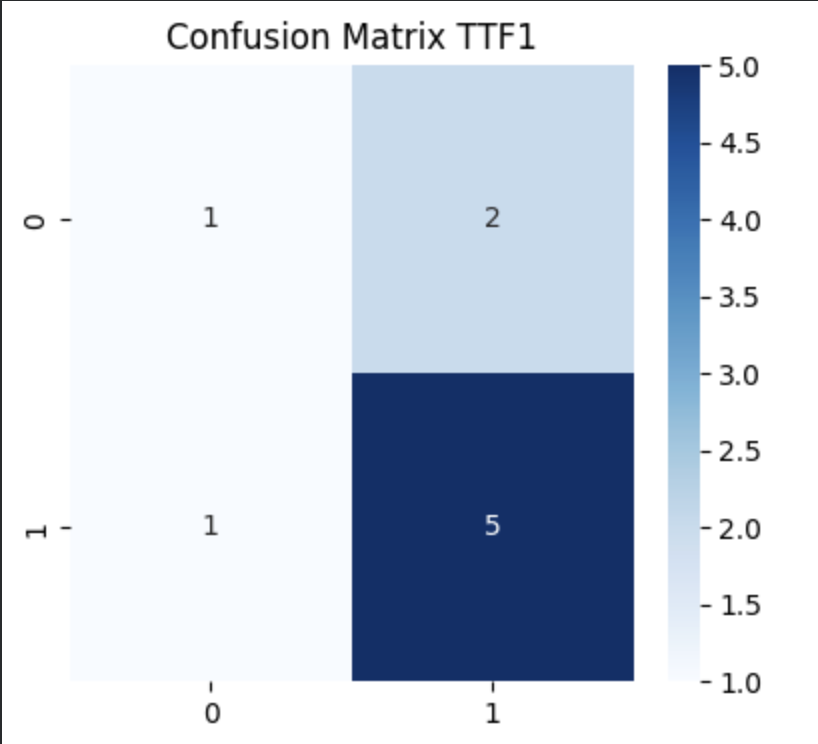
\includegraphics[width=0.5\textwidth]{Screenshot 2025-11-20 at 10.48.48.png}
    \caption{Confusion Matrix for TTF1.}
    \centering
    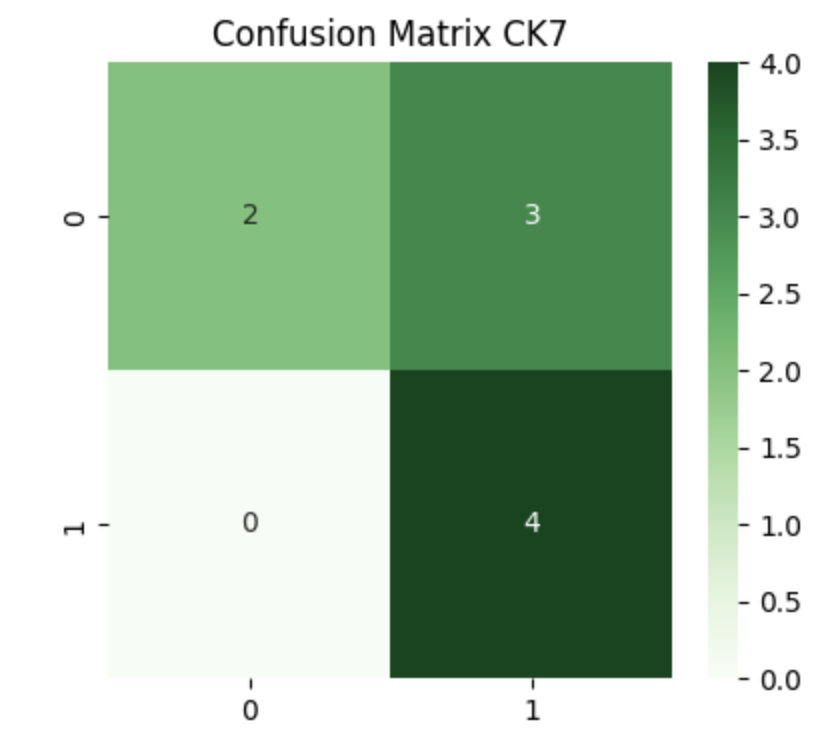
\includegraphics[width=0.5\textwidth]{Screenshot 2025-11-20 at 10.49.00.png}
    \caption{Confusion Matrix for CK7.}
    \centering
    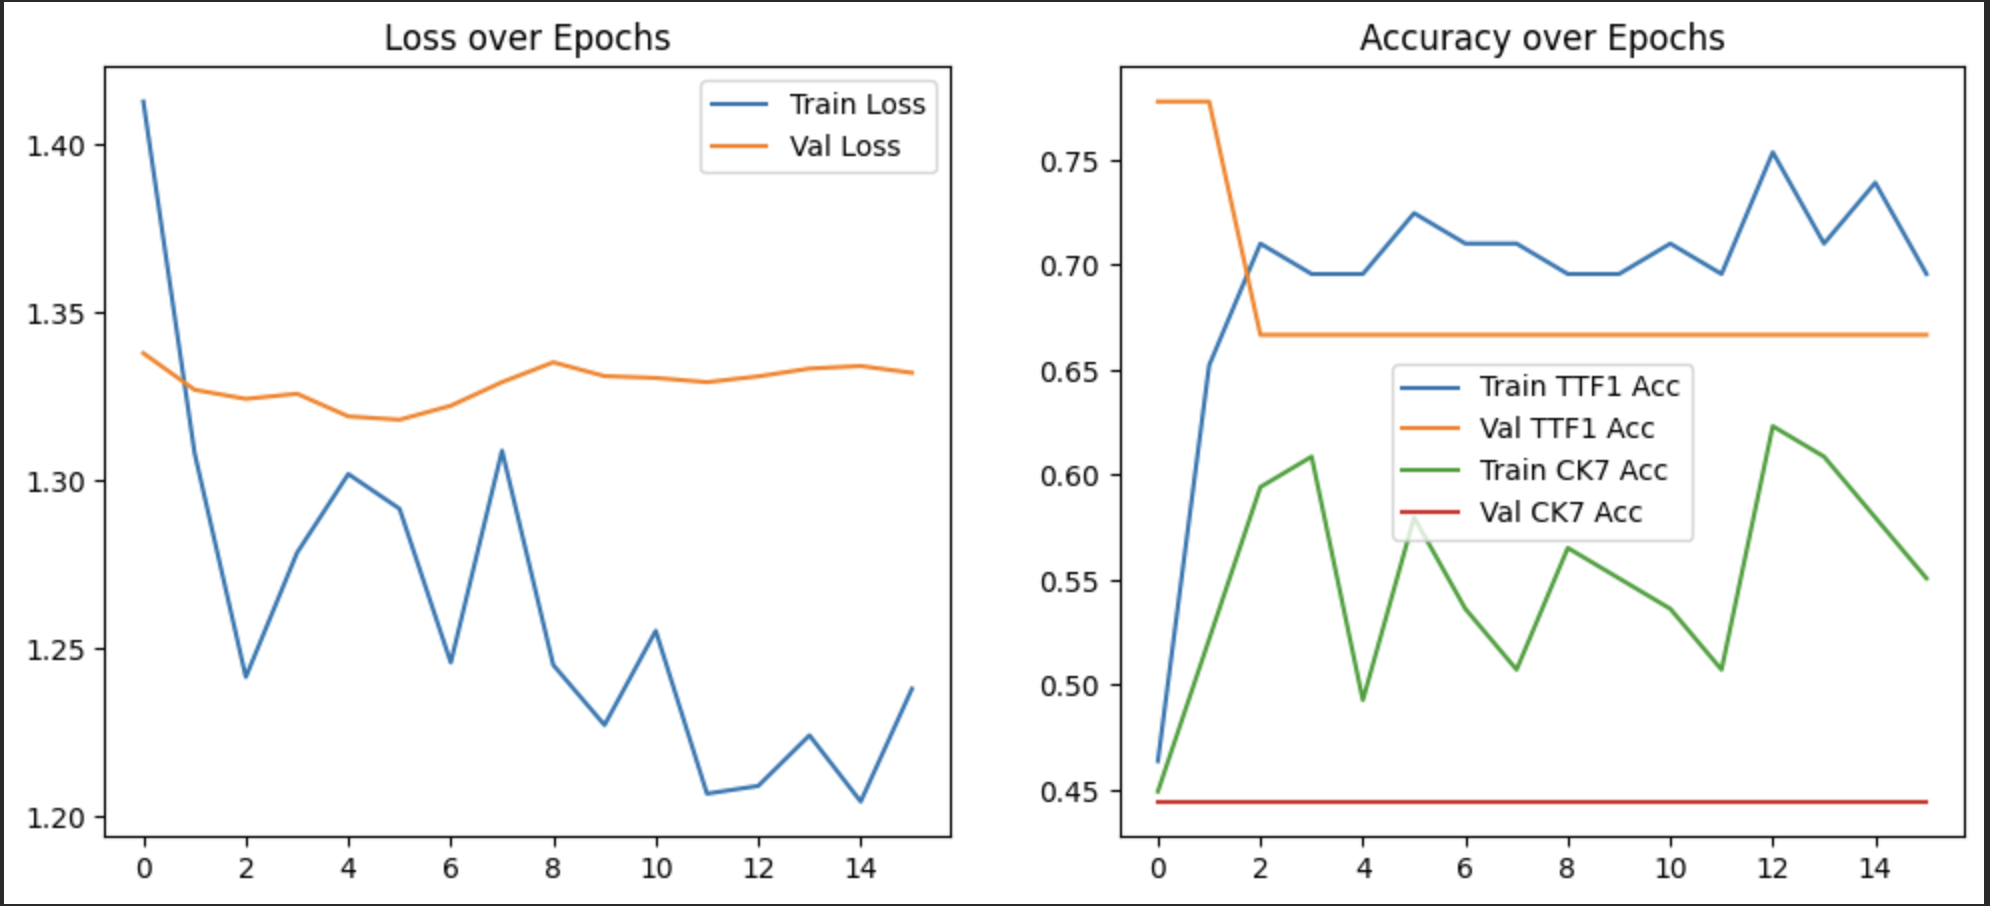
\includegraphics[width=1\textwidth]{Screenshot 2025-11-20 at 10.49.09.png}
\end{figure}

\subsubsection{Comparative Analysis}
\begin{itemize}
    \item \textbf{vs. Cropped CT (Exp 2)}: The performance was notably lower than the cropped experiments. This confirms that for molecular biomarker prediction, local texture resolution is paramount. The features defining TTF1/CK7 status are likely microscopic/textural rather than macroscopic/anatomical.
    \item \textbf{vs. Radiomics:} The handcrafted radiomics features (extracted from the full-resolution ROI) significantly outperformed this downsampled global approach.
\end{itemize}

\subsection{Conclusion of Experiment 6}
This experiment highlights the trade-off between context and resolution in medical imaging DL. For this specific task (genomic/proteomic biomarker prediction), the "signal" is concentrated within the tumor boundaries. Feeding the uncropped volume dilutes this signal, leading to suboptimal performance compared to ROI-based approaches. This validates the preprocessing pipeline (segmentation and cropping) used in Experiments 2-5 as a critical step.